\documentclass[oneside, 11pt]{article}

\usepackage[T1]{fontenc}
\usepackage[utf8]{inputenc}
\usepackage[dutch]{babel}

\usepackage{fouriernc}
\usepackage[detect-all, load-configurations=binary,
            separate-uncertainty=true, per-mode=symbol,
            retain-explicit-plus, range-phrase={ tot }]{siunitx}

\usepackage{setspace}
\setstretch{1.2}

\setlength{\parskip}{\smallskipamount}
\setlength{\parindent}{0pt}

\usepackage{geometry}
\geometry{marginparwidth=0.5cm, verbose, a4paper, tmargin=3cm, bmargin=3cm, lmargin=2cm, rmargin=2cm}

\usepackage{float}

\usepackage[fleqn]{amsmath}
\numberwithin{equation}{section}
\numberwithin{figure}{section}

\usepackage{graphicx}
\graphicspath{{Figures/}}
\usepackage{subfig}

\usepackage{tikz}
\usetikzlibrary{plotmarks}

\usepackage{fancyhdr}
\pagestyle{fancy}
\fancyhf{}
\rhead{\thepage}
\renewcommand{\footrulewidth}{0pt}
\renewcommand{\headrulewidth}{0pt}

\usepackage{relsize}
\usepackage{xspace}
\usepackage{url}

\newcommand{\figref}[1]{Figuur~\ref{#1}}

\newcommand{\hisparc}{\textsmaller{HiSPARC}\xspace}
\newcommand{\kascade}{\textsmaller{KASCADE}\xspace}
\newcommand{\sapphire}{\textsmaller{SAPPHiRE}\xspace}
\newcommand{\jsparc}{\textsmaller{jSparc}\xspace}
\newcommand{\hdf}{\textsmaller{HDF5}\xspace}
\newcommand{\aires}{\textsmaller{AIRES}\xspace}
\newcommand{\csv}{\textsmaller{CSV}\xspace}
\newcommand{\python}{\textsmaller{PYTHON}\xspace}
\newcommand{\corsika}{\textsmaller{CORSIKA}\xspace}
\newcommand{\labview}{\textsmaller{LabVIEW}\xspace}
\newcommand{\daq}{\textsmaller{DAQ}\xspace}
\newcommand{\adc}{\textsmaller{ADC}\xspace}
\newcommand{\adcs}{\textsmaller{ADC}s\xspace}
\newcommand{\Adcs}{A\textsmaller{DC}s\xspace}
\newcommand{\hi}{\textsc{h i}\xspace}
\newcommand{\hii}{\textsc{h ii}\xspace}
\newcommand{\mip}{\textsmaller{MIP}\xspace}
\newcommand{\hisparcii}{\textsmaller{HiSPARC II}\xspace}
\newcommand{\hisparciii}{\textsmaller{HiSPARC III}\xspace}
\newcommand{\pmt}{\textsmaller{PMT}\xspace}
\newcommand{\pmts}{\textsmaller{PMT}s\xspace}

\DeclareSIUnit{\electronvolt}{\ensuremath{\mathrm{e\!\!\:V}}}

\DeclareSIUnit{\unitsigma}{\ensuremath{\sigma}}
\DeclareSIUnit{\mip}{\textsmaller{MIP}}
\DeclareSIUnit{\adc}{\textsmaller{ADC}}

\DeclareSIUnit{\gauss}{G}
\DeclareSIUnit{\parsec}{pc}
\DeclareSIUnit{\year}{yr}



\title{Wireless connectie PC en Arduino}
\author{C.G.N. van Veen}
\docweerstation{2}{WW}
\version{1.0}

\begin{document}

\maketitle

\section{Weerstation}

\paragraph{Inleiding} Ons weerstation werkt en geeft ons de data die we
willen van het weer. Het is echter nog wel afhankelijk van een fysieke
verbinding met de pc. Omdat we in sommige gevallen op afstand willen
meten, kan het handig zijn om de data van het weerstation wireless naar
de PC te versturen. Dit heeft een aantal voordelen. We hoeven geen kabel
tussen PC en Arduino te trekken en we kunnen over grote afstand een nieuw
programma zenden naar de Arduino. Het nadeel dat we wel constante
voeding nodig hebben bij het station, gaan we ondervangen met een
zonnecel en backup batterij. 

\paragraph{Benodigdheden}
Om het geheel wireless te laten werken hebben we een aantal zaken nodig.
Het belangrijkste is de zend/ontvangmodule (APC220) module. Dit is een 
zend/ontvangmodule die makkelijk in te stellen is en makkelijk via een ander 
programma uit te lezen is.

\begin{itemize}  
    \item APC220 zendmodules (2x)    
    \item Arduino software
    \item USB to UART adapter
    \item APC programma
\end{itemize}

\begin{figure}
    \centering
    \subfloat[]{
        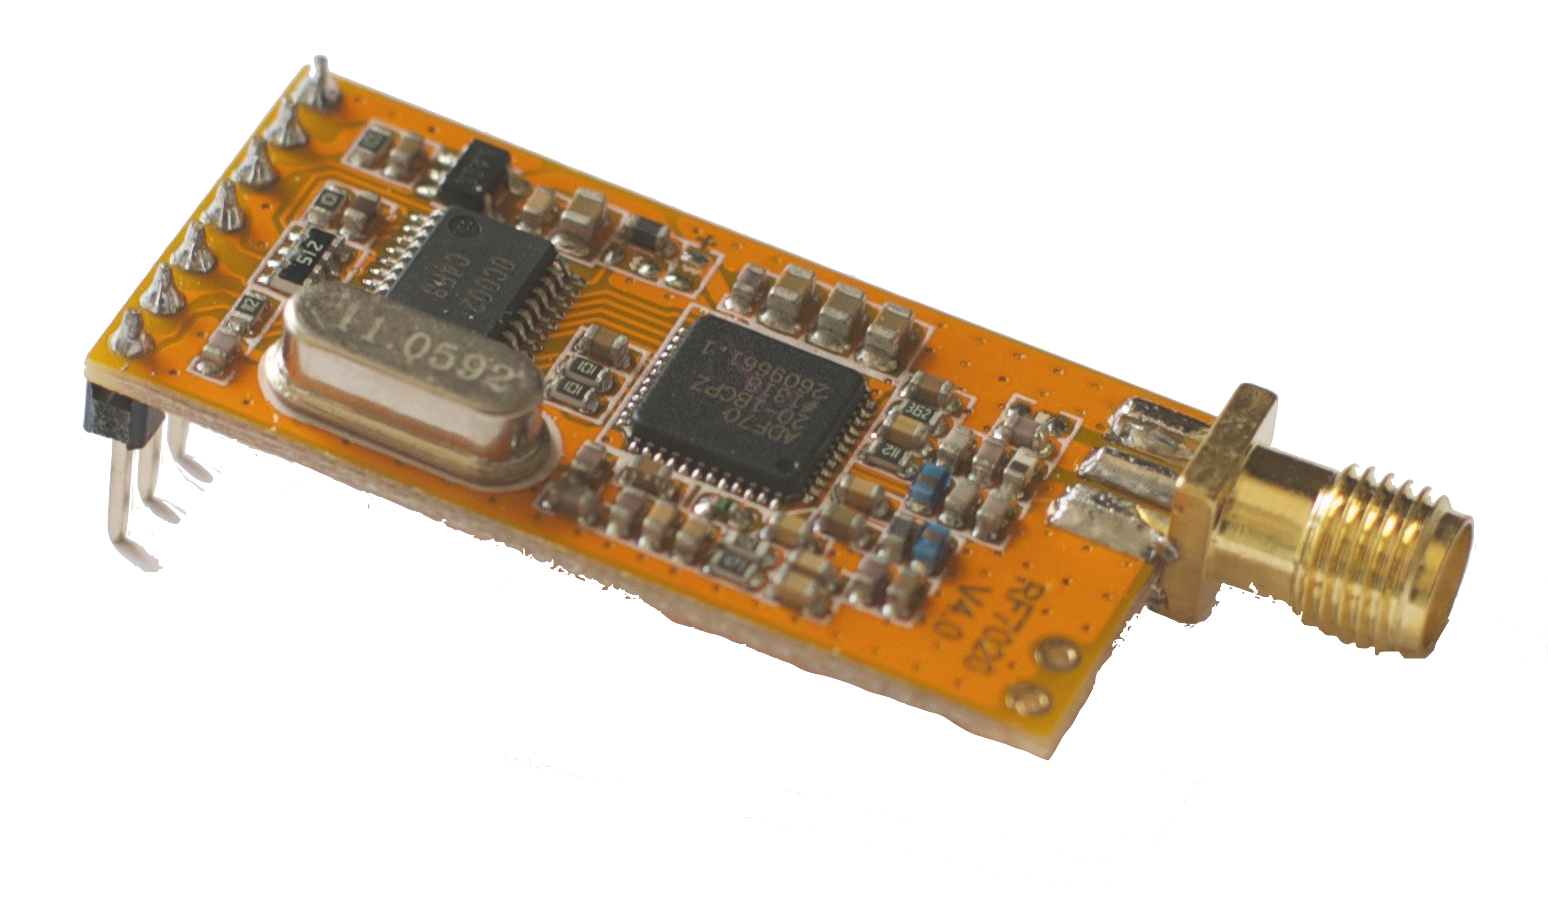
\includegraphics[width=.5\linewidth]{apc_receiver}
        \label{fig:apc_receiver}}
    \hfill
    \subfloat[]{
        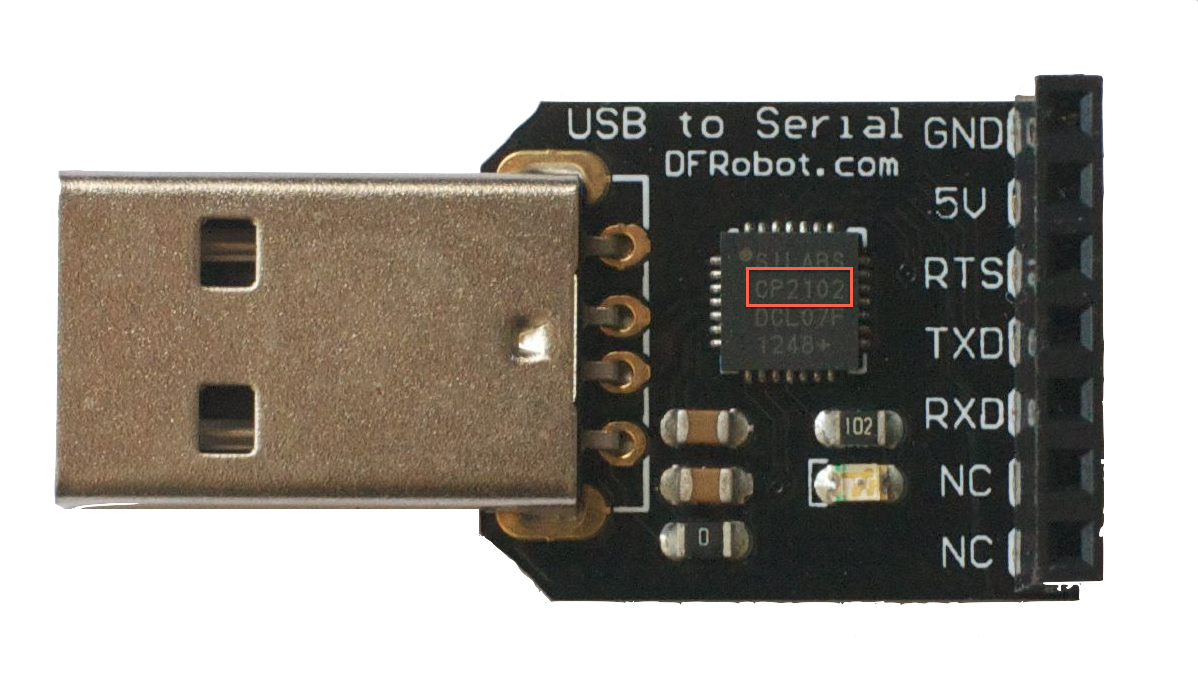
\includegraphics[width=.4\linewidth]{USB_adapter}
        \label{fig:USB_adapter}}
    \caption{Een APC zend of ontvanger module (a) en zijn USB adapter
    (b), in het rode kader het nummer van de chip (CP210), check of dit
    nummer in de driver beschrijving staat bij het downloaden van de
    driver van SILABS.}
\end{figure}

\section{APC module installeren}

\subsection{Zenden en ontvangen} Telemetrie is een technologie, die
ervoor zorgt dat data verzonden en ontvangen wordt. De data wordt
verzonden via radiogolven en door ontvangers opgevangen, bewaard en/of
bewerkt. Ons weerstation moet de data van de sensoren doorsturen naar de
\hisparc computer op school, zodat deze de data kan versturen. De
APC-220 module (zie \figref{fig:apc_receiver}), die we gebruiken is een
radio zender of ontvanger met een laag vermogen. Een van de modules
gebruiken we als ontvanger, die wordt dan ook aangesloten op de pc. De
andere wordt aangesloten op de Arduino en zal als zender fungeren. Het
bereik van de zender is 1 km in open lucht. De zender kan door muren heen
zenden, maar het verdient aanbeveling om het aantal muren tussen het
meetstation en de computer beperkt te houden. De zender kan zenden
tussen \SIrange{430}{440}{\MHz}. De default waarde is echter
\SI{434}{\MHz}. In tabel zie je mogelijke waarden die we gebruiken, de APC220 
kan zenden tussen \SI{418}{\MHz} en \SI{454}{\MHz}.
In Nederland mag er echter alleen tussen deze frequentiegrenzen door
zendamateurs informatie verzonden worden.


\subsection{APC-220 installeren}
De ontvanger zal gekoppeld moeten worden aan de computer. De computer heeft 
een driver nodig om te werken. We hebben een VCP (Virtual Com Port) driver nodig, 
die we kunnen downloaden van Silabs.com:
\url{http://www.silabs.com/products/mcu/Pages/USBtoUARTBridgeVCPDrivers.aspx.}
Download de juiste driver voor je besturingssysteem op de de gebruikte computer
en installeer deze. Zorg tijdens de installatie van de driver dat je de 
ontvangmodule nog niet in je pc hebt aangesloten.
Na installatie sluit je de APC module \figref{fig:APC_complete} aan op een 
USB ingang van de PC. Als Windows hem dan niet vind, verwijder de module en 
stop hem er opnieuw in.

Om de APC module te configureren gebruiken we de Arduino en een
programma 'apc220cfg.ino' dat we downloaden van de site van NAROM of van
de universiteit van Aalborg \footnote{NAROM is een
raketbasis/organisatie in Noorwegen die participeert in CANSAT (een
Europees project van de ESA). Zij hebben samen met de Aalborg
universiteit op basis van Arduino een pakket ontwikkeld waarmee een
CANSAT satelliet gemaakt kan worden. De CANSAT zendt draadloos data via
de APC-220 module. Andere tools om de APC-module te configureren bestaan
wel, maar geven veel problemen. Een voorbeeld van zo'n problematisch
programma is "RF-Magic". Gebruik Google met zoekterm 'apc220cfg.ino'} of van
Github/\hisparc. 

 
\begin{figure}
    \centering
    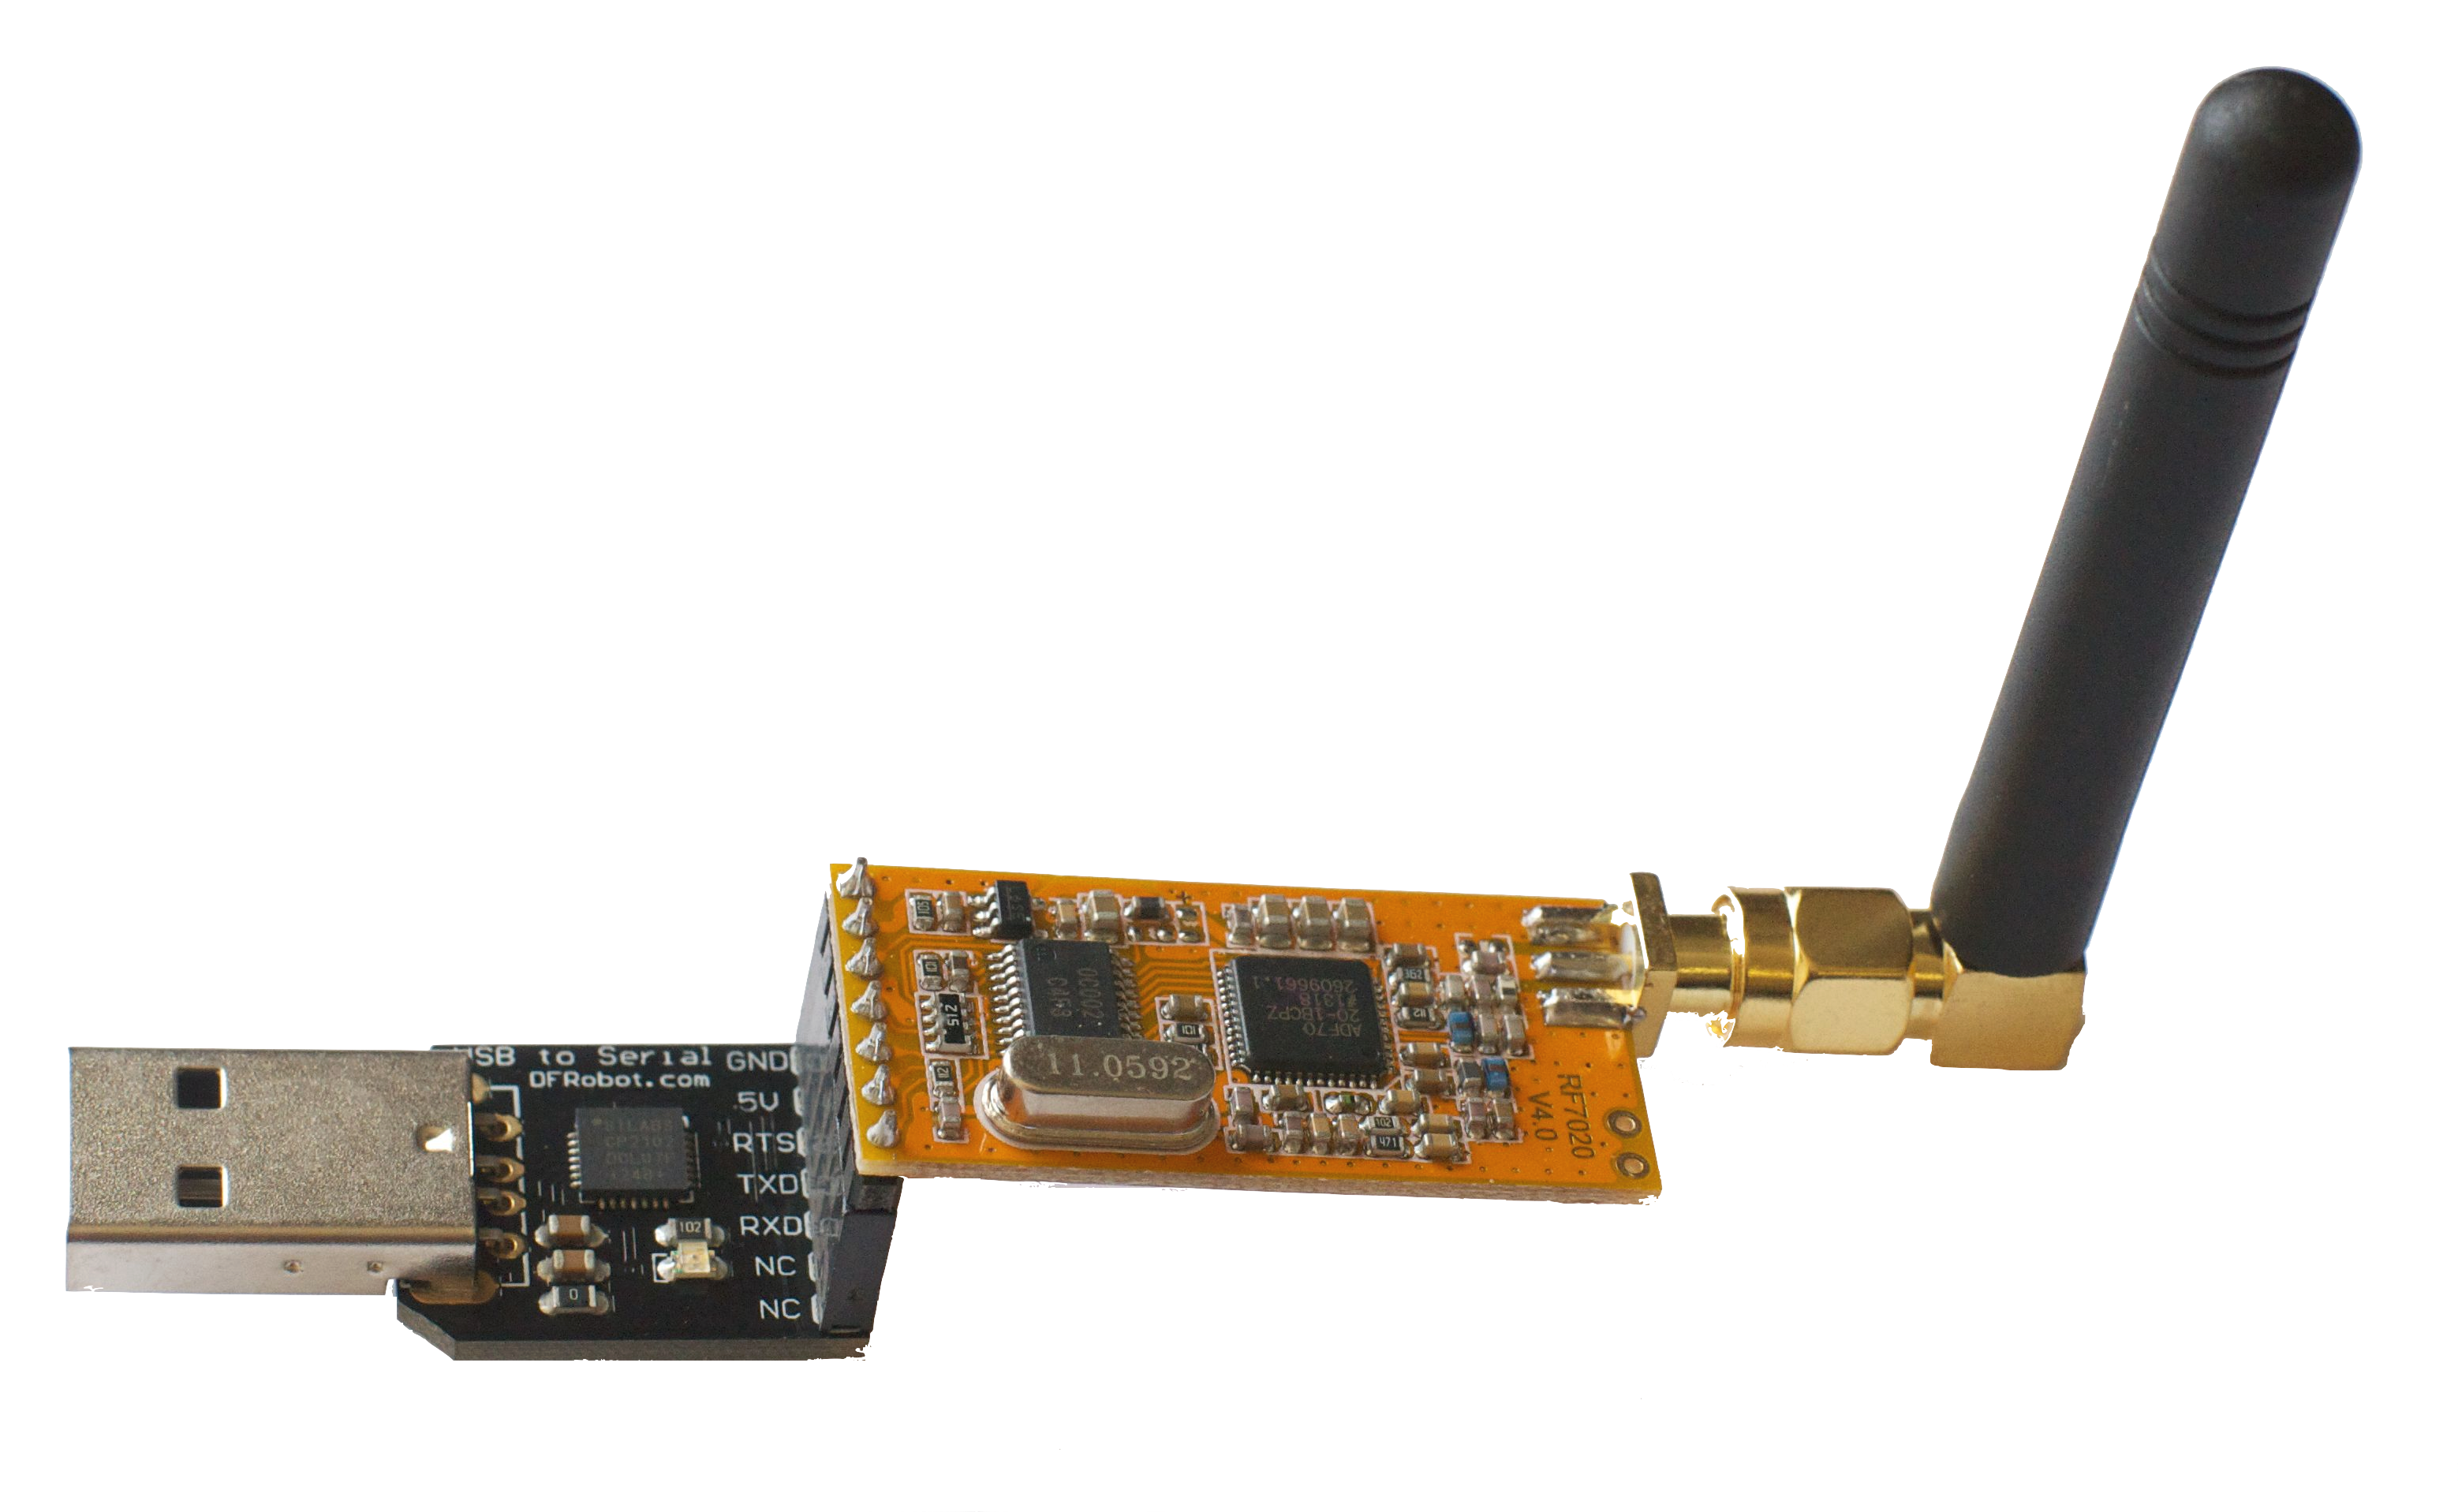
\includegraphics[width=0.60\textwidth]{APC_complete}
    \caption{De APC module op de aangesloten op de USB adapter.}
   \label{fig:APC_complete}
\end{figure}

\begin{figure}
    \centering
    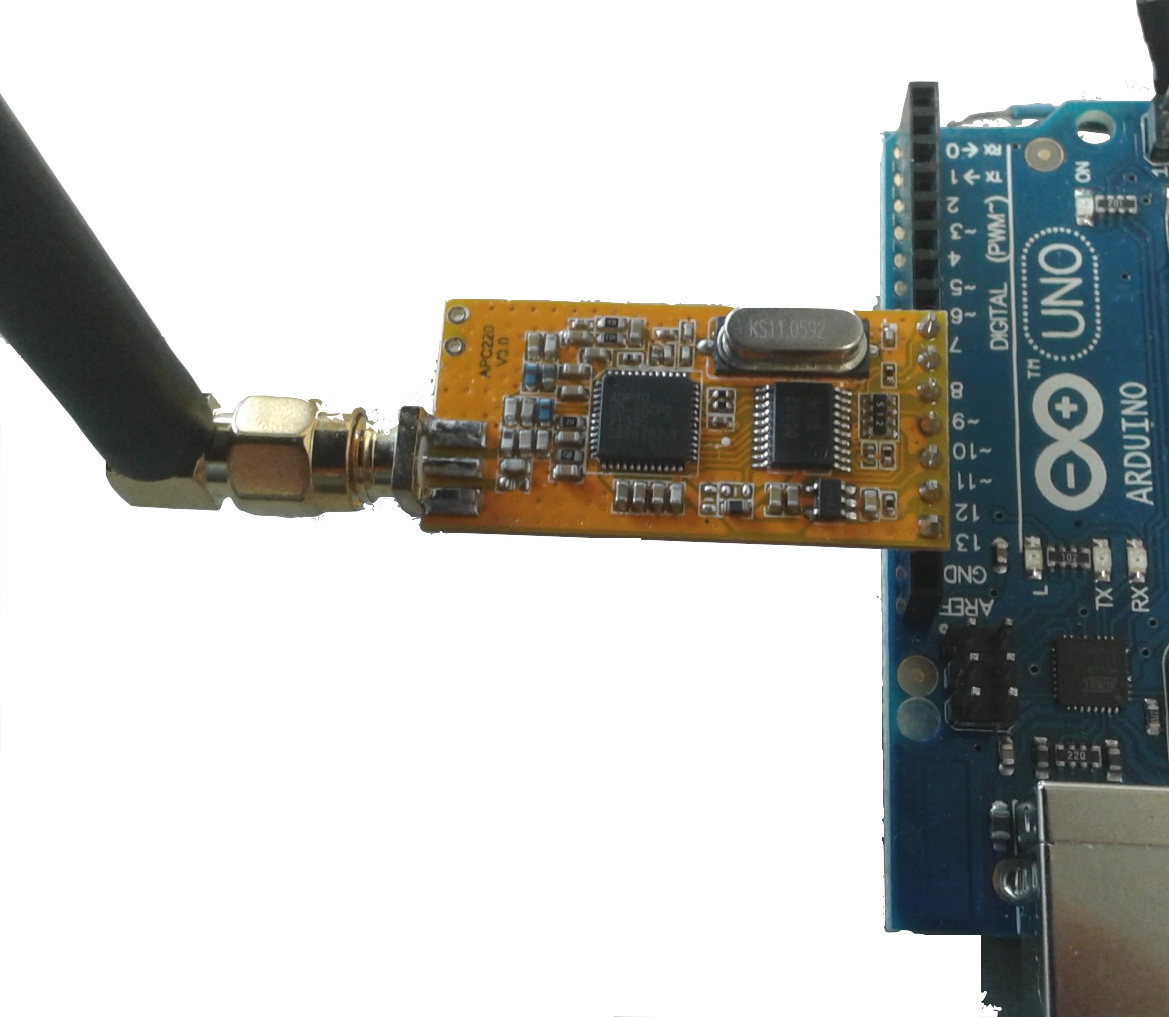
\includegraphics[width=0.5\textwidth]{APC220_configurat1}
    \caption{De APC module aangesloten op de Arduino om te configureren.
    Sluit de module aan op pin 8-13 en ground van de Arduino.}
   \label{fig:APC220_configurat1}
\end{figure}

\begin{figure}
    \centering
    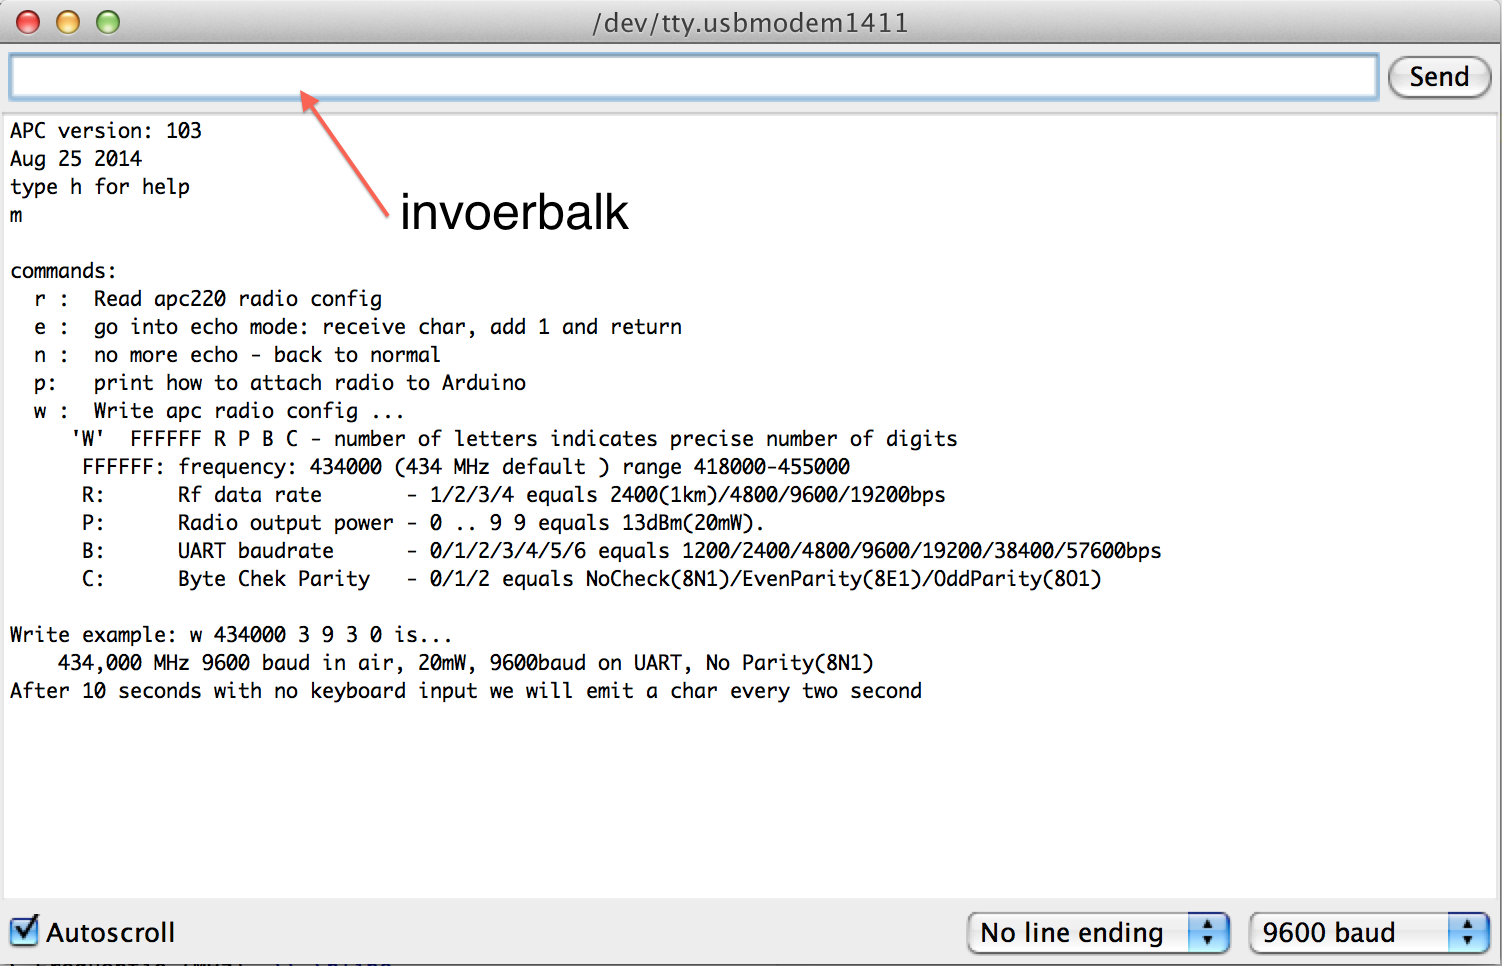
\includegraphics[width=0.60\textwidth]{scrshotConfigAPC}
    
    \caption{Screenshot van de "serial monitor", type 'm' in de invoerbalk
    van de serial monitor. Na het typen van 'm' wordt dit menu getoond.
    Type 'r' om de instellingen van de APC module uit te lezen. Type 'w'
    om de APC module configureren. Bepaal welke frequentie je wilt
    gebruiken voor transmissie en ontvangst uit tabel \ref{table:frequenties}.
    Voorbeeld: w 434150 3 9 3 0 (denk aan de spaties) betekent: write
    frequentie \SI{434150}{\MHz} met 9600 bps in lucht, met een zendvermogen van
    \SI{20}{\milli\watt} ontvangen van data met 9600 bps over UART zonder parity
    check.}
   
   \label{fig:scrshotConfigAPC}
\end{figure}

\begin{figure}
    \centering
    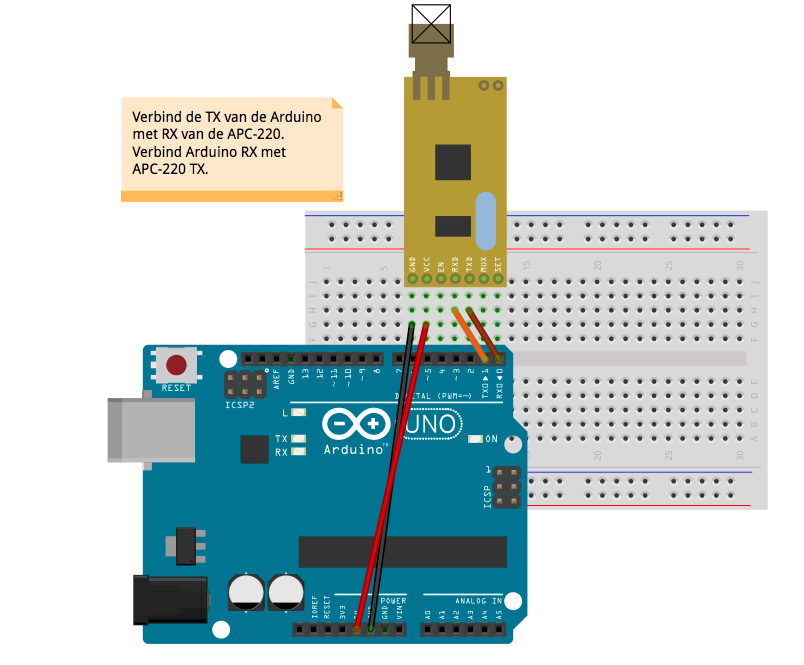
\includegraphics[width=0.80 \textwidth]{APCTXRX}
    \caption{De APC module aangesloten op de Arduino om te zenden.}
   \label{fig:APCTXRX}
\end{figure}

\subsection{Configureren van de APC-220}

Start nu Arduino software op en open het programma 'apc220cfg.ino'. We
willen nu de frequentie gaan instellen waarmee de module zendt en
ontvangt. Upload het programma naar de Arduino voordat je de APC module
aansluit op de Arduino. Maak nu de USB kabel los en verwijder eventueel
de voeding van de Arduino. Plaats nu de APC module op de Arduino zoals
is aangegeven in \figref{fig:APC220_configurat1}. De APC moet zo
geplaatst worden dat de pinnen van de APC in pin 8-13 en ground van de
Arduino zitten. Sluit de Arduino nu opnieuw aan met behulp van de USB
kabel en open de "Serial Monitor" van Arduino. Type in de invoerbalk van
de "Serial Monitor", 'm'. Dan opent het menu wat in
\figref{fig:scrshotConfigAPC} te zien is. Met dit menu kun je de APC-module
configureren. Het invoeren van de letter 'r' geeft de huidige
configuratie van de APC module weer. Bepaal met behulp van tabel
\ref{table:frequenties} op welke frequentie je beide modules wilt laten
werken. Beide modules moeten op dezelfde frequentie werken. Voer dan je
keuze in. Bijvoorbeeld de invoer: w 434790 3 9 3 0 staat voor: write
frequentie \SI{434150}{\MHz} met 9600 bps in lucht en
\SI{20}{\milli\watt} 9600 bps wegschrijven over UART zonder parity check.
Herhaal deze stap voor de andere APC module. Belangrijk is dat de Baudrate op 
9600 staat en paritycheck 'none' is.



\begin{center}
\begin{table}
    \begin{tabular}{ | l | l | }
    \hline
    Frequentie (MHz) & Frequentie (MHz)  \\ \hline
    433050 & 433950     \\ \hline
    433100 & 434000     \\ \hline
    433150 & 434050     \\ \hline
    433200 & 434100     \\ \hline
    433250 & 434150     \\ \hline
    433300 & 434200     \\ \hline
    433350 & 434250     \\ \hline
    433400 & 434300     \\ \hline
    433450 & 434350     \\ \hline
    433500 & 434400     \\ \hline
    433550 & 434450     \\ \hline
    433600 & 434500     \\ \hline
    433650 & 434550     \\ \hline
    433700 & 434600     \\ \hline
    433750 & 434650     \\ \hline
    433800 & 434700     \\ \hline
    433850 & 434750     \\ \hline
    433900 & 434790     \\ \hline
   \end{tabular}
   \caption{tabel met frequenties: Volgens \cite{Radio} mag in Nederland
   dit bereik van radiofrequenties gebruikt worden voor telemetrie op
   een vermogen van \SI{10}{\milli\watt}}
   \label{table:frequenties}
\end{table}
\end{center}

\subsection{Zenden en ontvangen met de APC module}

We hebben nu de modules zo geconfigureerd dat ze in principe klaar zijn
om te zenden en ontvangen. Nu moeten we ons weerprogramma weer uploaden
naar de Arduino. Sluit de USB kabel aan op de Arduino en upload het
weerprogramma. Run het programma, kijk in de serial monitor van de
arduino software of er data verschijnt. Sluit de serial monitor. We gaan
nu wireless meten.

Sluit een voeding aan op de Arduino.
We sluiten de APC-modules aan zoals in \figref{fig:APCTXRX} (let op de
verbindingen RX $\longleftrightarrow$ TX) en plaatsen de APC module met UART
in de USB ingang van de pc. De Arduino software zal de UART vinden en
geeft ook de poort aan, waar deze zit. Ga naar \emph {"Tools"},
\emph{"Serial Port"}. Daar vind je de poort waar de UART  zit. Het adres
van deze poort is nodig om met een andere programmeertaal (in ons
geval: Python) de gegevens van het weerstation uit te lezen.  

Een voorbeeld programma in Python om data van het weerstation uit te lezen.

\begin{minted}{python}
    import sys, serial
    import time
    from time import sleep
   
    
    def main():
    strPort = '/dev/tty.SLAB_USBtoUART' # Adres APC-UART module.
    ser = serial.Serial(strPort, baudrate=9600, parity=serial.PARITY_NONE, 
        bytesize=serial.EIGHTBITS, stopbits=serial.STOPBITS_ONE, timeout=1.0)
    
    while True:
    try:

      line = ser.readline()
      print line
      time.sleep(10)
 
    except KeyboardInterrupt:
      print 'exiting'
      break
    if __name__ == '__main__':
    main()
\end{minted}

In het volgende document gaan we het programma aanpassen om daadwerkelijk de 
data naar de database van \hisparc te schrijven.

\section{Wireless weerstation plaatsen}

\subsection{Behuizing Arduino weerstation} Het weerstation moet kunnen
meten aan het weer, dus de behuizing moet voldoen aan de eigenschappen
van een weerhuisje, zoals waterdicht, wind doorlatend en niet in de
volle zon opgesteld. Daarbij komt dat de Arduino gevoed moet worden. Als
er buiten in de buurt van het weerstation een voeding is, dan is het
voedingsprobleem zo opgelost. Anders kan een oplossing met een zonnecel
en een oplaadbare batterij uitkomst bieden. Bijvoorbeeld de 'Solar
MintyBoost' of zelf een combinatie maken van een zonnecel en een
oplaadbare batterij. Er zijn wat printplaatjes te koop die een zonnecel
combineren met een oplaadbare batterij zoals de 'USB LiPoly Charge'.

  


 
\begin{thebibliography}{9}
    \bibitem{CANSAT}
        NAROM, 2013 \emph{The CANSAT BOOK 2013-edition}, 
        CANSAT project
    \bibitem{Radio}
    Agentschap Telecom, 2012 \emph{Vergunningsvrije radiotoepassingen}, 
    Ministerie van Economische zaken, Landbouw en Innovatie
\end{thebibliography}


\end{document}
